\begin{hyperbolicbox}{Lattices $\Lambda\subset\C$}
    \small
    \begin{defi}
        A \textit{lattice} $\Lambda$ in the complex plane is an additive discrete subgroup of $\C$. \cite{LozanoEC}
        Equivalently, $\Lambda\subset\C$ is a lattice if there are $p,q\in\C$ linearly independent over $\R$, i.e. $\frac{p}{q}\notin\R$, such that
        $$
        \Lambda=\group{p,q}=\set{ap+bq:a,b\in\Z}
        $$
    \end{defi}
    As an example, the figure below shows the lattice $\group{\frac{1}{2}+\frac{3}{2}i,\frac{3}{2}+\frac{3}{2}i}$.
    \begin{figure}[H]
        \centering
        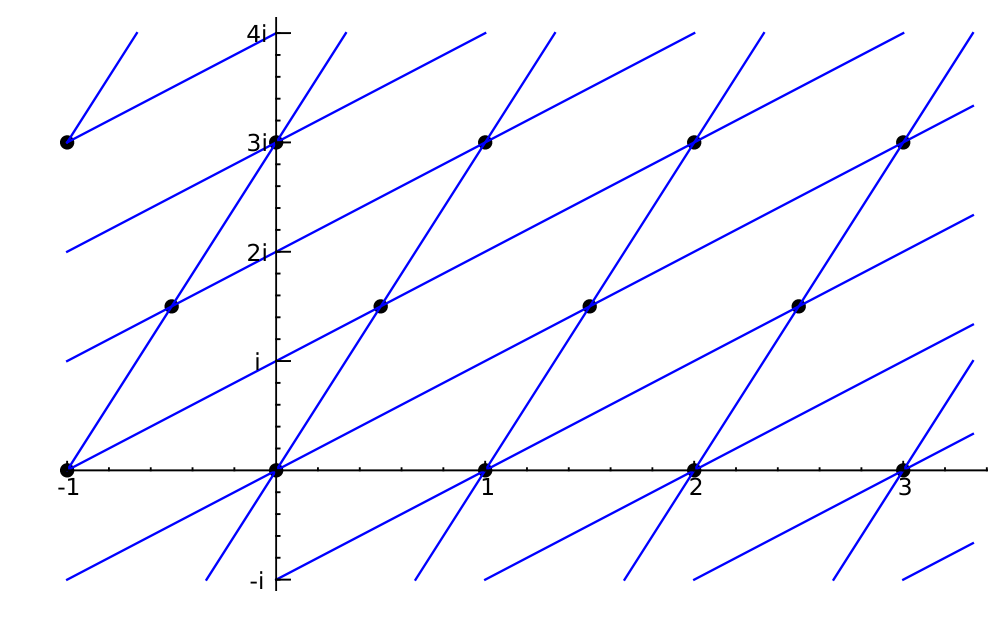
\includegraphics[width=0.5\linewidth]{Images/lat1.png}
    \end{figure}
    For a lattice $\Lambda=\group{p,q}$, one can prove that the parallelogram
    $$
    \mathcal{F}=\set{ap+bq:0\leq a,b<1}
    $$
    is a fundamental domain for $\C/\Lambda$.
    \begin{thm}\cite{LozanoEC}\label{thm5}
        Let $\Lambda=\group{p,q}$ and $\Lambda'=\group{p',q'}$ be two lattices with $\frac{p}{q},\frac{p'}{q'}\in\H$. We have $\Lambda=\Lambda'$ if and only if there is a matrix $M\in\operatorname{SL}(2,\Z)$ such that 
        $$
        \begin{pmatrix}
            p'\\q'
        \end{pmatrix}=M
        \begin{pmatrix}
            p\\q
        \end{pmatrix}
        $$
    \end{thm}
\end{hyperbolicbox}